\documentclass[conference]{IEEEtran}
\usepackage{graphicx}
\usepackage{amsmath,amssymb}
\usepackage{booktabs}
\usepackage{cite}
\usepackage{url}
\usepackage[hidelinks]{hyperref}
\setlength{\textfloatsep}{6pt}
\setlength{\dbltextfloatsep}{6pt}
\setlength{\abovedisplayskip}{3pt}
\setlength{\belowdisplayskip}{3pt}
\newcommand{\ns}{$^\circ$}

\begin{document}

\title{ASR-Aware Unified Fusion of Three Speech Enhancers for Noise Event Removal on Vaani}

\author{\IEEEauthorblockN{Manish Joshi \qquad Neeraj Singh Aithani}
\IEEEauthorblockA{Team Hydra, IndoML Datathon 2026, Track 2: Noise Event Removal}}

\maketitle

\begin{abstract}
Track 2 removes noise events from Indic field speech, scored by SI-SDR plus 100$\times$ the word error rate reduction
($\Delta$WER) of the organisers' SraVaani-1.0 ASR. Cleaner waveforms alone do not give the ASR back its words, so our
main novelty is to train speech enhancers \emph{through the frozen scoring ASR's own decoder} (encoder distance and
transcript likelihood, also on 12--18\,s recordings matching the test clips' length) and to fuse three public
enhancers of different families (MossFormerGAN, a 104M band-split RNN, TF-Locoformer) per time-frequency cell with a
deletion-weighted word-error loss. Every clip takes the same path. The final entry scores Combined 19.897 (SI-SDR
15.793\,dB, $\Delta$WER $+4.104$\,pp) on the Phase 2 board.
\end{abstract}
\end{abstract}

\section{Training Data and Preprocessing}
\textbf{The task and the organiser data.} A test clip is either \emph{synthetic} (clean speech with noise events
pasted in, scored by SI-SDR and $\Delta$WER) or \emph{natural} (a field recording, scored by $\Delta$WER). The
validation release has 695 synthetic pairs (clean and noisy, 4.5\,s median) and 1,806 natural recordings with
transcripts, in 27 languages. A fixed hash of the speaker id sets 30\% of speakers aside: their 209 pairs never train
the models we evaluate with (the \emph{held-out protocol}, 486 training pairs), giving honest scores and unseen inputs
for the fusion; our final MossFormerGAN and BSRNN are retrained on all 695 (TF-Locoformer stays on 486: retraining it
on all pairs scored lower on the board). Natural clips are never trained on; a fixed 30\% hash sample of them (555
clips, 7,834 words) measures natural $\Delta$WER.

\textbf{Noise events.} Noisy minus clean at the annotated spans gives 2,213 events (23\,min, 7 categories), used
only to build training mixtures.

\textbf{External speech.} Test clips are long (13\,s median) single-speaker recordings, while the validation pairs
are 4.5\,s from few speakers, so we needed more clean speech: Vaani-transcription-part~\cite{vaani}, the corpus the
competition clips come from, and IndicVoices-R~\cite{ivr}. From them we cut clean \emph{beds} (recordings onto which
noise events are pasted) that pass Silero-VAD~\cite{silero} and TorchAudio-SQUIM~\cite{squim} checks
(Table~\ref{tab:data}).

\textbf{Data use and fairness.} The competition allows external data when disclosed; Table~\ref{tab:data} lists all
of it. (a)~\emph{No competition recordings in external data.} Vaani-transcription-part is the competition's source
corpus, so before any use we deleted every clip named like a competition clip (validation, Track 1 training, Phase 1
test: 98,653 names) and every clip from the same recording as a validation or Phase 1 test clip (9,931 recordings). Phase 2 test clips are anonymised, so we compared content instead: the ASR
transcripts of all 3,178 test clips against those of all external speech we trained on (1,450 long beds and all 5,000
fresh2 clips). No test clip shares 30\% of its 8-word sequences with any of them (the largest, 20\%, is a speaker
counting). This rules out reused recordings, though a speaker could appear in both.
(b)~\emph{No test audio in training}; the only test information used is distribution-level (clip lengths and blind SNR
estimates), to size our simulated clips. (c)~\emph{Noise events.} Synthetic clips share a common event pool, so test
clips may contain events from the validation release we train on; a control model trained without the held-out pairs'
events scored the same on them (18.64 vs 18.64\,dB after 4k steps, with identical curves throughout), so the models do not rely on having heard a specific event.
Nothing at inference stores, matches or subtracts events.

\textbf{Making training examples.} A training crop (2\,s for MossFormerGAN, 4\,s otherwise) is a real pair with
probability 0.5, else a clean reference plus 1--3 random events at an SNR drawn from the real pairs. Each step also adds
a \emph{long stream} micro-batch of 12--18\,s long beds with events pasted as the organisers do (Poisson 0.5 events/s,
log-normal gain, median 0.93, $\sigma{=}0.8$), for the ASR losses only. For all training audio the ASR losses' target is SraVaani's own
greedy transcript of the clean speech. Simulated sets: \emph{fresh2} joins 1--4 beds of one speaker into 8--18\,s clips on
beds no member saw, to train the fusion; \emph{valset} glues the 209 held-out pairs' clean references (reused across clips) into 1,200 test-like clips
(33.8k words), to compare training choices; \emph{valset\_long} pastes events onto one long Vaani recording from each of
360 speakers kept out of all training beds, for evaluation.

\begin{table}[t]
\caption{Every dataset used and its role (beds: clean recordings onto which events are pasted). No test audio,
external noise or TTS speech is used.}
\label{tab:data}
\centering\scriptsize
\setlength{\tabcolsep}{2pt}
\resizebox{\columnwidth}{!}{%
\begin{tabular}{@{}lllc@{}}
\toprule
Data (source, version) & Used & How & Final \\
\midrule
\multicolumn{4}{@{}l}{\emph{Organiser data (Vaani validation release)}} \\
Synthetic pairs & 695 pairs, 1.0\,h & member training (209 held out) & yes \\
Noise events (noisy $-$ clean) & 2,213, 0.4\,h & training mixtures only & yes \\
Natural recordings & 555 of 1,806 & evaluation only & no \\
\multicolumn{4}{@{}l}{\emph{External data (public, gated); every competition clip and recording removed first}} \\
Vaani-transcription-part~\cite{vaani} (\texttt{d2acadf}) & 1,450 long beds, 5.7\,h & long stream, all members & yes \\
 & 710 beds, 1.4\,h & fusion mixtures (908 clips) & yes \\
IndicVoices-R~\cite{ivr} (\texttt{5f4495c}) & 2,793 beds, 6.5\,h & fusion mixtures (1,592 clips) & yes \\
 & 198\,h more & member training (Table~\ref{tab:tried}) & no \\
\multicolumn{4}{@{}l}{\emph{Simulated from the above (noise events pasted onto clean speech)}} \\
fresh2 & 2,500 clips, 9.9\,h & fusion training (153 dev) & yes \\
valset & 1,200 clips, 4.2\,h & member screening; fusion training & yes \\
valset\_long & 360 clips, 1.3\,h & evaluation only & no \\
\bottomrule
\end{tabular}}
\end{table}

\section{Proposed Method}
\textbf{Preliminary observations.} (1) \emph{A cleaner waveform does not give back the words}: on valset, at equal
SI-SDR (15.8\,dB), speech with the events merely turned down 20\,dB recovers 92\% of the \emph{ceiling} (the $\Delta$WER
of the clean reference), our first fixed blend of enhancers only 32\%. (2) \emph{The test is longer, not harder}:
similar estimated SNR but 13\,s clips against 4.5\,s, and SraVaani's encoder output for a 2\,s crop differs from the
same speech inside the full clip (cosine distance 0.24). (3) \emph{Diversity comes from model
families, not seeds}: two seeds of a model make nearly the same errors (correlation 0.95--0.99), a new family's errors
correlate only 0.69 with our existing ensemble. (4) \emph{Lost words are mostly deletions} (71\% then; 89\% in the final system).

\textbf{System overview} (Fig.~\ref{fig:system}). Three enhancers (\emph{members}, Table~\ref{tab:models}) each
clean the clip, a small \emph{fusion} network decides in every time-frequency cell how much to trust each, and a fixed
post-processing step finishes.

\textbf{Novelty and contributions.} Prior work matches a recogniser's features (mimic loss~\cite{mimic}), adds part
of the noisy input back to limit ASR-harmful artefacts~\cite{obsadd,artifacts}, and trains recognisers with sampled
minimum-word-error (MWER) losses~\cite{shannon,mwer}. We contribute: (i)~\emph{enhancer training on the scoring
recogniser's own decoder}: SraVaani's encoder distance and its transducer likelihood of the target transcript (via a
forward recursion we wrote for words cut at crop edges) each improved $\Delta$WER by 0.24--0.61\,pp on all three model
families we tried (MP-SENet, MossFormerGAN, BSRNN) at no SI-SDR cost, and a sampled, deletion-weighted MWER risk
(REINFORCE~\cite{reinforce}) added $+0.26$\,pp in the fusion (Table~\ref{tab:tried}); (ii)~\emph{a long-recording
stream} (12--18\,s, the test clips' length) for these losses, the largest training gain ($+1.47$\,pp on valset over
two seeds, $+0.38$\,pp on valset\_long); (iii)~\emph{a learned per-cell fusion of three model families with a bounded
input add-back}, trained through the ASR losses and the post-processing, gaining 0.74\,dB SI-SDR over a fixed mix of
the same members at equal $\Delta$WER (Table~\ref{tab:main}).

\begin{figure}[t]
\centering
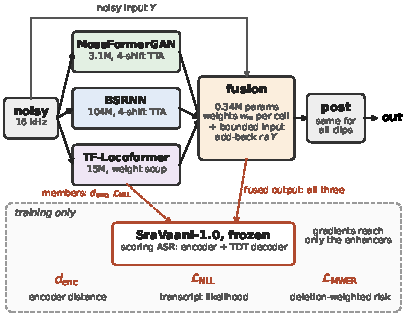
\includegraphics[width=0.76\columnwidth]{../figures/system.pdf}
\caption{Every clip takes the same path (top); in training only, the frozen scoring ASR scores members and fusion (bottom).}\vspace{-2pt}
\label{fig:system}
\end{figure}

\begin{table*}[t]
\caption{What we tried, each change against its own control on a set the compared models never trained on (sim =
valset; long = valset\_long; h/o = 209 held-out pairs, fusions 2-fold out-of-fold). $\Delta$WER: change in pp
[95\% CI], \ns{} CI includes zero; one seed unless noted. Board: change in Combined of one upload (noise $\pm0.1$). MFGAN = MossFormerGAN,
TF-Loco = TF-Locoformer. MP-SENet: an early member, later dropped. A change was kept when its $\Delta$WER or SI-SDR interval excluded zero and the board did not drop; $^\dagger$kept for simplicity at equal
$\Delta$WER, or only as one of three averaged models.}
\label{tab:tried}
\centering\scriptsize
\setlength{\tabcolsep}{3.2pt}
\resizebox{\textwidth}{!}{%
\begin{tabular}{@{}lllllrc@{}}
\toprule
Change & Model & Set & $\Delta$WER (pp) & SI-SDR (dB) & Board & Kept \\
\midrule
\multicolumn{7}{@{}l}{\emph{Training through the ASR (observations 1, 2, 4)}} \\
Encoder distance, weight 30 & MFGAN & sim & $+0.30$ [0.06, 0.53] & $0.00$ & & yes \\
Encoder distance, weight 30, 2k; 8k steps & MP-SENet & sim & $+0.33$; $+0.54$ [0.24, 0.81] & $0.00$ & $+0.18$ (2k) & yes \\
+ transcript NLL, weight 2.5 & BSRNN 38M; 104M; MFGAN & sim & $+0.61$ [0.36, 0.85]; $+0.43$ [0.22, 0.65]; $+0.24$ [0.03, 0.50] & $+0.05$; $0.00$; $0.00$ & & yes \\
Long single-recording stream (2 seeds) & BSRNN 38M & sim; long & $+1.47$ [1.18, 1.78]; $+0.38$ [0.14, 0.62] & $+0.30$; -- & & yes \\
Long stream also on MFGAN and TF-Loco & 3 members & long & $+0.33$ [0.07, 0.60] & $+0.23$ & $+0.11$ & yes \\
MWER (weight 3) on a member & TF-Loco & long & $-0.17$\ns & -- & $+0.02$ & soup$^\dagger$ \\
MWER in the fusion & fusion & long & $+0.26$ [0.10, 0.43] & $-0.02$ & $+0.04$ & yes \\
\multicolumn{7}{@{}l}{\emph{Members, fusion and data (observation 3)}} \\
Learned per-cell fusion vs fixed mix (first version) & fusion & h/o & $+0.30$\ns & $+0.06$ [0.02, 0.10] & $+0.13$ & yes \\
Add TF-Locoformer (error corr.\ 0.69 vs 0.82--0.90) & mix & long & -- & $+0.79$ (351/360 clips) & $+1.37$ & yes \\
Three members instead of eight earlier candidates & fusion & long & $-0.04$\ns & $-0.11$ & $+0.02$ & yes$^\dagger$ \\
Weight soup of three fine-tunes & TF-Loco & h/o & $+0.17$\ns & $+0.085$ [0.056, 0.118] & $+0.03$ & yes \\
198\,h more clean speech (IndicVoices-R) & 4 families & sim; h/o & $+0.10$\ns (MP-SENet) & $-0.05$ to $-0.17$ & & no \\
\multicolumn{7}{@{}l}{\emph{Other targets and post-processing}} \\
Keep the input where the model left the audio unchanged & post & sim & $+0.08$ & $+0.44$ & $+0.05$ & yes \\
Louder output (peak normalisation) & post & sim & $+0.71$ [0.47, 0.97] & $0.00$ & $-0.19$ & no \\
\bottomrule
\end{tabular}}
\end{table*}

\textbf{Members and their losses.} Each member is fine-tuned with
\begin{equation}
\mathcal{L}=-\text{SI-SDR}(\hat{s},s)+30\,d_{\text{enc}}(\hat{s},s)+2.5\,\mathcal{L}_{\text{NLL}}+\lambda\,\mathcal{L}_{\text{MWER}},
\end{equation}
plus $15\times$ its compressed-spectrum L1 loss for MossFormerGAN; only the enhancer learns. $d_{\text{enc}}$ is the
mean per-frame cosine distance between SraVaani's encoder outputs for enhanced and clean speech. SraVaani decodes with a
token-and-duration transducer (TDT~\cite{tdt}); $\mathcal{L}_{\text{NLL}}$ is its per-token negative log-likelihood of
the target transcript given the enhanced audio, with paths free to start and end within 240\,ms of a crop edge.
$\mathcal{L}_{\text{MWER}}$ samples four transcripts per window of 8\,s or more and raises the likelihood of those with
fewer word errors than average (a deletion counts 2; REINFORCE); $\lambda{=}3$ in the fusion and one TF-Locoformer
fine-tune, else 0. \emph{Training} (AdamW, cosine decay, weight EMA; exact stages in the repository's configs):
MossFormerGAN (2\,s crops) and BSRNN (4\,s) first learn SI-SDR (and L1), then add the encoder loss, the NLL and the
long stream in turn; TF-Locoformer (4\,s) trains 20k steps from MERL's checkpoint with all three, then three 4k-step
fine-tunes (with MWER, without, louder events) are averaged into one model (a weight soup~\cite{soup}).

\begin{table}[t]
\caption{Pretrained models in the final system (models tried and dropped are listed in the repository).}
\label{tab:models}
\centering\scriptsize
\setlength{\tabcolsep}{2.5pt}
\resizebox{\columnwidth}{!}{%
\begin{tabular}{@{}lll@{}}
\toprule
Model (source, version) & Params & Role \\
\midrule
MossFormerGAN\_SE\_16K (ClearVoice~\cite{clearvoice} 0.1.2, \texttt{dcb1b20}) & 3.1M & member 1, 4-shift TTA \\
BSRNN large-double, VCTK+DNS+WHAMR!~\cite{espnetse} & 104M & member 2, 4-shift TTA \\
\multicolumn{3}{@{}l}{\quad {\tiny\texttt{wyz/vctk\_dns2020\_whamr\_bsrnn\_large\_double\_noncausal@da049f2}, \texttt{91epoch.pth}}} \\
TF-Locoformer M, DNS-2020 (MERL~\cite{loco}) & 15M & member 3, weight soup \\
\multicolumn{3}{@{}l}{\quad {\tiny\texttt{github.com/merlresearch/tf-locoformer@7a61546}, \texttt{egs2/dns\_ins20}, \texttt{valid.loss.ave\_5best.pth}}} \\
SraVaani-1.0~\cite{sravaani} (rev.\ \texttt{f5dd535}) & -- & frozen loss, transcripts \\
Silero-VAD 6.2.3~\cite{silero}, SQUIM (torchaudio 2.9.0)~\cite{squim} & -- & bed screening \\
\bottomrule
\end{tabular}}
\end{table}

\textbf{Fusion.} Member outputs $X_m$ are scaled to the input $Y$ by least squares (512-point STFT, hop 128).
Eight residual blocks of dilated 3$\times$3 convolutions (64 channels) see the log powers of the members, $Y$ and a
fixed mix $B=\sum_m w^0_m X_m$, and each member's phase and level relative to $B$; per cell they predict softmax
weights $w_m$ (from $w^0=(0.2,0.35,0.45)$) and a small complex add-back $r$ of the noisy cell
($|\Re r|,|\Im r|\le0.2$), allowed only where the mix changed the input:
\begin{equation}
\hat{S}=\textstyle\sum_m w_m X_m + r\,a\,Y,\quad a=\min\!\big(1,|Y-B|/|Y|\big).
\end{equation}
It learns on held-out-protocol copies of the members (486 pairs only) run over fresh2, the 209 held-out pairs and
valset, so its inputs are unseen; 3,000 steps with the member losses plus MWER, through the post-processing (its masks
held fixed). At
inference the all-pair members replace these copies (a swap not measured separately).

\textbf{Inference and post-processing.} MossFormerGAN and BSRNN average over four input delays (0, 41, 83, 124
samples), a test-time augmentation (TTA) known as the shift trick~\cite{demucs}; long clips are decoded in overlapping
windows (TF-Locoformer 8\,s, BSRNN 20\,s, MossFormerGAN 10\,s). A light post-processing step changes the fusion output
by only $-41$\,dB (median on the test clips): since enhancers alter clean speech slightly even where no event is
present, it keeps the model output where it changed the audio (smoothed difference above 1.5\% of its maximum, widened
150\,ms) and the input elsewhere, mutes stretches 50\,dB below the clip level and limits peaks to 0.99 ($+0.44$\,dB,
$+0.08$\,pp on valset). Every clip gets the same processing; nothing inspects a clip to choose its path.

\section{Results and Conclusion}
\textbf{Main results} (Table~\ref{tab:main}). Combined $=$ SI-SDR~\cite{sisdr} on synthetic clips $+\,100\cdot\Delta$WER
(noisy minus enhanced word error rate, pooled over all 3,178 test clips); local comparisons are paired, on sets the
compared models never trained on, with 95\% clip-bootstrap intervals. Each enhancer alone already improves both metrics, TF-Locoformer
most. The learned fusion adds 0.74\,dB SI-SDR over the fixed mix of the same members (both with post-processing) at
the same $\Delta$WER, and recovers 53\% of the ceiling; the share is the same (52--56\%) for clips with little, medium and much
of their length under events. On the board, the final entry gains $+11.66$\,pp on synthetic clips, more than locally because the test's
synthetic clips lose more words to noise, and $+0.54$\,pp on natural clips, where locally no system changes word error
measurably; Combined is 19.897.

\begin{table}[t]
\caption{Main results, out of sample (members alone without post-processing; fixed mix and fusion with it), and the
final board entry.}
\label{tab:main}
\centering\scriptsize
\setlength{\tabcolsep}{2.5pt}
\resizebox{\columnwidth}{!}{%
\begin{tabular}{@{}lccc@{}}
\toprule
 & \multicolumn{2}{c}{valset\_long} & natural \\
System & SI-SDR (dB) & $\Delta$WER (pp) & $\Delta$WER (pp) \\
\midrule
Noisy input & $-5.60$ & 0 & 0 \\
MossFormerGAN alone & 13.51 & $+2.46$ & $-0.06$ \\
BSRNN-104M alone & 14.49 & $+2.87$ & $-0.08$ \\
TF-Locoformer alone & 15.22 & $+4.13$ & $-0.11$ \\
Fixed mix $w^0$ & 15.30 & $+3.98$ & $+0.05$ \\
\textbf{Learned fusion (ours)} & \textbf{16.05} & $+4.06$ [3.46, 4.76] & $-0.05$ [$-0.38$, 0.27] \\
\midrule
Speech intact, events at $-20$\,dB & 14.39 & $+6.54$ & -- \\
Clean speech (the ceiling) & -- & $+7.59$ & -- \\
\midrule
\textbf{Board, final entry} & \textbf{15.79} & $+11.66$ (synthetic) & $+0.54$ \\
\multicolumn{4}{@{}l}{\quad Combined $= 15.793 + 4.104$ (pooled $\Delta$WER) $= \mathbf{19.897}$} \\
\bottomrule
\end{tabular}}
\end{table}

\textbf{Where words are still lost.} Of the words our system still loses on test-length clips, 89\% are deletions.
On valset\_long, speech left intact under turned-down events keeps 86\% of the ceiling at a \emph{lower} SI-SDR than ours, so the limit
is setting the right gain in each cell under loud events, not leftover noise. In natural clips, word error is 25.4\% in
clear speech, 26.8\% under local events (2,033 words) and 32.7\% under background noise (749 words): removing all
noise could gain only about 1\,pp of the 7,834 words' error.

\textbf{Validity.} The final entry is the best of 45 uploads (history in \texttt{docs/BOARD\_HISTORY.md}; uploads
before the organisers' one-pipeline rule handled natural clips separately, every later one does not), so 19.90 is
optimistic; one upload resolves only about $\pm0.1$ Combined, so small steps rest on the local intervals of
Table~\ref{tab:tried} (louder output won locally but lost on the board).

\textbf{Code and checkpoints} (training, data preparation, inference, a reproduction guide; final and every
intermediate checkpoint):\\
{\footnotesize\url{https://github.com/mcjoshi/asr-aware-noise-event-removal}}\\
{\footnotesize\url{https://huggingface.co/manishjoshiai/asr-aware-noise-event-removal}}

\textbf{Conclusion.} Three enhancers trained against the scoring ASR's own objectives and fused per cell reach
Combined 19.90 with every clip processed identically.

\def\IEEEbibitemsep{0pt plus .5pt}
\begin{thebibliography}{99}
\scriptsize
\bibitem{vaani} ARTPARK and IISc, ``Project Vaani,'' \url{https://huggingface.co/datasets/ARTPARK-IISc/Vaani-transcription-part}, 2025.
\bibitem{ivr} A. Sankar \emph{et al.}, ``IndicVoices-R: Unlocking a massive multilingual multi-speaker speech corpus for scaling Indian TTS,'' NeurIPS Datasets and Benchmarks, 2024.
\bibitem{silero} Silero Team, ``Silero VAD,'' \url{https://github.com/snakers4/silero-vad}, 2024.
\bibitem{squim} A. Kumar \emph{et al.}, ``TorchAudio-Squim: Reference-less speech quality and intelligibility measures in TorchAudio,'' ICASSP, 2023.
\bibitem{mimic} D. Bagchi \emph{et al.}, ``Spectral feature mapping with mimic loss for robust speech recognition,'' ICASSP, 2018.
\bibitem{obsadd} K. Kinoshita \emph{et al.}, ``Improving noise robust automatic speech recognition with single-channel time-domain enhancement network,'' ICASSP, 2020.
\bibitem{artifacts} K. Iwamoto \emph{et al.}, ``How bad are artifacts?: Analyzing the impact of speech enhancement errors on ASR,'' Interspeech, 2022.
\bibitem{shannon} M. Shannon, ``Optimizing expected word error rate via sampling for speech recognition,'' Interspeech, 2017.
\bibitem{mwer} R. Prabhavalkar \emph{et al.}, ``Minimum word error rate training for attention-based sequence-to-sequence models,'' ICASSP, 2018.
\bibitem{reinforce} R. J. Williams, ``Simple statistical gradient-following algorithms for connectionist reinforcement learning,'' Machine Learning, 1992.
\bibitem{tdt} H. Xu \emph{et al.}, ``Efficient sequence transduction by jointly predicting tokens and durations,'' ICML, 2023.
\bibitem{soup} M. Wortsman \emph{et al.}, ``Model soups: averaging weights of multiple fine-tuned models improves accuracy without increasing inference time,'' ICML, 2022.
\bibitem{clearvoice} ModelScope, ``ClearerVoice-Studio,'' \url{https://github.com/modelscope/ClearerVoice-Studio}, 2025.
\bibitem{espnetse} J. Yu and Y. Luo, ``Efficient monaural speech enhancement with universal sample rate band-split RNN,'' ICASSP, 2023.
\bibitem{loco} K. Saijo \emph{et al.}, ``TF-Locoformer: Transformer with local modeling by convolution for speech separation and enhancement,'' IWAENC, 2024.
\bibitem{sravaani} ARTPARK and IISc, ``SraVaani-1.0,'' \url{https://huggingface.co/ARTPARK-IISc/SraVaani-1.0}, 2026.
\bibitem{demucs} A. D\'efossez \emph{et al.}, ``Music source separation in the waveform domain,'' arXiv:1911.13254, 2019.
\bibitem{sisdr} J. Le Roux \emph{et al.}, ``SDR -- half-baked or well done?,'' ICASSP, 2019.
\end{thebibliography}

\end{document}
